\documentclass{standalone}
%\usepackage{import}
%\subimport{.../}{preamble}
\usepackage{tikz, graphicx, cmbright}
\begin{document}

\begin{tikzpicture}
\fontsize{10pt}{1em}\selectfont
\node [above right] at (0, 0) {\includegraphics[scale=1.3]{tip_alignment_diagram.png}};

\node at (0.2, 2) {$x$};
\node at (0.6, 0.85) {$y$};
\node at (2, 0.2) {$z$};

\node at (4.45, 2.55) {$R$};
%\node at (4.0, 3.2) {$dz$};
%\node [left] at (4.15, 0.8) {$dx,dy$};
\node [align=left, below right] at (0.9,3) {\textbf{tip 1}:\\$k_{01}^z, m_1, \omega_{01}$\\$\beta_{01}$};
\node [align=right, below left] at (10.5,2.6) {\textbf{tip 2}:\\$k_{02}^z, m_2, \omega_{02}$\\$\beta_{02}$};

\node at (5.8, 4.1) {$V(t)=V_0\cos(\omega_{01} t/2)$};

\node at (5.68, 0.95) {$d_0$};
\node at (5.55, 0.55) {$d(t)$};
\node at (7.35, 1.85) {$A_{ov}$};

%\fontsize{9pt}{1em}\selectfont
\node at (5, 3.7) {$z_{1}(t)$};
\node at (5.35, 3.35) {$z_{01}$};
\node [right] at (5.7, 3.35) {$z_{02}=0$};

\end{tikzpicture}

\end{document}